% ============================================================
%  ChurnGuard AI — IEEE Double-Column Conference Report
%  Compile order: pdflatex → bibtex → pdflatex → pdflatex
% ============================================================

\documentclass[conference]{IEEEtran}
\IEEEoverridecommandlockouts

% ── Packages ─────────────────────────────────────────────────
\usepackage[numbers]{natbib}
\usepackage{amsmath,amssymb,amsfonts}
\usepackage{algorithm}
\usepackage{algorithmic}
\usepackage{graphicx}
\usepackage{textcomp}
\usepackage{xcolor}
\usepackage{url}
\usepackage{booktabs}
\usepackage{multirow}
\usepackage{listings}
\usepackage{float}
\usepackage{caption}
\usepackage{microtype}
\usepackage{cleveref}

\lstset{
  basicstyle=\ttfamily\footnotesize,
  breaklines=true,
  frame=single,
  captionpos=b,
  keywordstyle=\color{blue},
  commentstyle=\color{gray},
  xleftmargin=2pt,
  xrightmargin=2pt,
  aboveskip=10pt,
  belowskip=10pt
}

% ── Title & Authors ──────────────────────────────────────────
\begin{document}

\title{Project 5: Customer Churn Prediction and \\ Agentic Retention Strategy System}

\author{
  \IEEEauthorblockN{
  Ananya,
  Aditya Bijalwan,
  Mahek Motwani,
  Khush Kanubhai Chaudhari
  }
  \IEEEauthorblockA{\textit{Team: Infera}\\
  Course: Artificial Intelligence / Machine Learning \\
  April 2026}
}

\maketitle

% ── Abstract ────────────────────────────────────────────────
\begin{abstract}
Customer churn is one of the most critical challenges in the
telecommunications industry, with acquisition costs estimated at five to
seven times the cost of retention. This paper presents
\textit{ChurnGuard AI}, a two-milestone system that combines a classical
supervised machine learning pipeline with a modern agentic AI layer.
Milestone 1 trains and compares three classifiers — Logistic Regression,
Random Forest, and Gradient Boosting — on the IBM Telco Churn dataset
(7,043 records, 30 engineered features). Gradient Boosting achieves the
best balanced performance (Accuracy~79.77\%, Recall~73.73\%,
ROC-AUC~0.860) and is deployed as the production model.
Milestone 2 extends the system with a LangGraph-based agentic workflow
that uses a large-language model (LLM) via the Groq API, SHAP
explainability, and a Retrieval-Augmented Generation (RAG) pipeline to
produce personalised, structured retention strategies. Two extension
features are included: a one-click PDF report generator and a batch
analytics dashboard. The entire system is served through a Streamlit web
application that provides actionable, interpretable insights for business
stakeholders.
\end{abstract}

\begin{IEEEkeywords}
churn prediction, logistic regression, gradient boosting, SHAP
explainability, large language models, LangGraph, RAG, Streamlit,
telecom analytics, customer retention.
\end{IEEEkeywords}

% ============================================================
\section{Introduction}
% ============================================================

Customer churn — the voluntary discontinuation of a service subscription
— represents a significant revenue risk for telecom operators. Industry
research consistently shows that acquiring a new customer costs five to
seven times more than retaining an existing one \cite{reichheld1990zero}.
With the global telecommunications market projected to exceed
\$2.5 trillion by 2026 \cite{statista2024telecom}, even a 1\% reduction
in monthly churn can translate to millions of dollars in retained revenue.

Traditional approaches to churn management rely on static segmentation
rules or periodic batch reports, which fail to anticipate individual
customer behaviour with sufficient granularity. Recent advances in
machine learning (ML) have demonstrated that predictive models trained on
historical customer data can identify at-risk customers weeks before they
cancel, enabling timely, personalised interventions
\cite{vafeiadis2015comparison}.

This project addresses the problem on two levels:

\begin{enumerate}
  \item \textbf{Milestone 1 — Predictive ML Pipeline:} Design, train, and
        compare multiple classifiers on the IBM Telco Churn dataset;
        deploy the best model in a Streamlit dashboard with risk scoring
        and feature explainability.
  \item \textbf{Milestone 2 — Agentic AI Advisor:} Wrap the ML output in
        a LangGraph agent that calls an LLM (Groq, Llama-3 70B) and a RAG
        retriever to generate customer-specific, actionable retention
        strategies.
\end{enumerate}

The remainder of this paper is organised as follows: Section II reviews
related work; Section III describes the methodology (data, preprocessing,
and models); Section IV presents results and analysis; Section V discusses
the Milestone 2 agentic architecture; Section VI concludes with
limitations and future directions.

% ============================================================
\section{Related Work}
% ============================================================

Churn prediction has been extensively studied in the supervised learning
literature. Vafeiadis et al.~\cite{vafeiadis2015comparison} benchmarked
nine classifiers on a telecom dataset and found that Support Vector
Machines and ensemble methods consistently outperformed Logistic
Regression in raw accuracy, yet noted that interpretability constraints
often favour simpler models in production.

Umayaparvathi and Iyakutti~\cite{umayaparvathi2016attribute} demonstrated
that attribute selection substantially improves churn model performance,
reducing noise and overfitting in high-dimensional one-hot-encoded feature
spaces — a finding directly applicable to the 30-feature space used here.

More recently, Krishna et al.~\cite{kirui2013predicting} highlighted that
\textit{Recall} is the preferred business metric for churn, since false
negatives (missed churners) carry greater economic cost than false
positives. This motivates the use of \texttt{class\_weight=\char`"balanced\char`"}
in our Logistic Regression and optimal threshold selection.

On the interpretability frontier, Lundberg and Lee~\cite{lundberg2017shap}
introduced SHAP (SHapley Additive exPlanations), a game-theoretic
framework that provides consistent, locally faithful feature attributions.
SHAP is integrated into ChurnGuard AI to explain individual predictions
to non-technical stakeholders.

The application of LLMs to structured business data for recommendation
generation is an emerging area. Lewis et al.~\cite{lewis2020rag} proposed
Retrieval-Augmented Generation (RAG) as a mechanism to ground LLM outputs
in factual, domain-specific knowledge — the architecture adopted in
Milestone 2.

% ============================================================
\section{Methodology}
% ============================================================

\subsection{Dataset Description}

The \textbf{IBM Telco Customer Churn} dataset \cite{kaggle_telco} contains
records for 7,043 residential customers of a fictional US telecom provider.
Each row represents one customer and includes 21 raw attributes spanning
four domains:

\begin{itemize}
  \item \textit{Demographics} — \texttt{gender}, \texttt{SeniorCitizen},
        \texttt{Partner}, \texttt{Dependents}
  \item \textit{Service subscriptions} — \texttt{PhoneService},
        \texttt{MultipleLines}, \texttt{InternetService},
        \texttt{OnlineSecurity}, \texttt{OnlineBackup},
        \texttt{DeviceProtection}, \texttt{TechSupport},
        \texttt{StreamingTV}, \texttt{StreamingMovies}
  \item \textit{Account details} — \texttt{tenure}, \texttt{Contract},
        \texttt{PaperlessBilling}, \texttt{PaymentMethod},
        \texttt{MonthlyCharges}, \texttt{TotalCharges}
  \item \textit{Target} — \texttt{Churn} (Yes / No)
\end{itemize}

The dataset is \textbf{class-imbalanced}: 26.5\% of customers churned
(1,869 records) versus 73.5\% who did not (5,174 records), as illustrated
in Figure~\ref{fig:churn_dist}.

\begin{figure}[H]
  \centering
  
\includegraphics[width=0.45\textwidth]{figures/churn_distribution.png}
  \caption{Class distribution of the target variable \texttt{Churn}.
           The dataset exhibits a 73.5\,:\,26.5 imbalance requiring
           class-weight compensation during training.}
  \label{fig:churn_dist}
\end{figure}

\subsection{Preprocessing}

The raw dataset required the following preprocessing steps, applied
consistently across all models:

\begin{enumerate}
  \item \textbf{Drop identifier:} \texttt{customerID} was removed (no
        predictive signal).
  \item \textbf{Type coercion:} \texttt{TotalCharges} was cast from
        \textit{object} to \textit{float64}; 11 rows with whitespace-only
        values were set to \texttt{NaN}.
  \item \textbf{Imputation:} All missing numerical values were filled with
        the column \textit{median} (robust to outliers); categorical
        missing values were filled with the column \textit{mode}.
  \item \textbf{Target encoding:} \texttt{Churn} was binarised
        (Yes$\to$1, No$\to$0).
  \item \textbf{One-Hot Encoding:} All categorical features were
        one-hot-encoded with \texttt{drop=\char`"first\char`"} to avoid
        perfect multicollinearity, yielding \textbf{30 final features}.
  \item \textbf{Train/test split:} 80\,/\,20 stratified split
        (\texttt{random\_state=42}), preserving class proportions in both
        partitions.
  \item \textbf{Standardisation:} \texttt{StandardScaler} was fit
        \textit{only} on the training set and applied to both splits,
        preventing data leakage.
\end{enumerate}

The final feature matrix has shape $(7{,}043 \times 30)$ before splitting.
The 30 features after one-hot encoding are listed in
Table~\ref{tab:features}.

\begin{table}[H]
\centering
\caption{Final feature set after one-hot encoding (30 features)}
\label{tab:features}
\renewcommand{\arraystretch}{1.1}
\begin{tabular}{ll}
\toprule
\textbf{Type} & \textbf{Feature names} \\
\midrule
Numerical (4) & \texttt{SeniorCitizen}, \texttt{tenure}, \\
              & \texttt{MonthlyCharges}, \texttt{TotalCharges} \\
\midrule
Binary (5)    & \texttt{gender\_Male}, \texttt{Partner\_Yes}, \\
              & \texttt{Dependents\_Yes}, \texttt{PhoneService\_Yes}, \\
              & \texttt{PaperlessBilling\_Yes} \\
\midrule
Service (14)  & \texttt{MultipleLines\_*}, \texttt{InternetService\_*}, \\
              & \texttt{OnlineSecurity\_*}, \texttt{OnlineBackup\_*}, \\
              & \texttt{DeviceProtection\_*}, \texttt{TechSupport\_*}, \\
              & \texttt{StreamingTV\_*}, \texttt{StreamingMovies\_*} \\
\midrule
Contract (2)  & \texttt{Contract\_One year}, \texttt{Contract\_Two year} \\
\midrule
Payment (3)   & \texttt{PaymentMethod\_Credit card}, \\
              & \texttt{PaymentMethod\_Electronic check}, \\
              & \texttt{PaymentMethod\_Mailed check} \\
\bottomrule
\end{tabular}
\end{table}

\subsection{Feature Engineering}

No hand-crafted composite features were added; the feature space after
one-hot encoding was sufficient. Feature \textit{selection} was evaluated
using the Logistic Regression coefficients and Gradient Boosting
importances. The top-5 features by absolute coefficient magnitude in
the final LR model are:

\begin{enumerate}
  \item \texttt{Contract\_Two year} (strong retention signal, negative
        coefficient)
  \item \texttt{tenure} (negative — longer customers less likely to churn)
  \item \texttt{InternetService\_Fiber optic} (positive — higher risk)
  \item \texttt{TotalCharges} (negative at scale — proxy for loyalty)
  \item \texttt{PaperlessBilling\_Yes} (positive correlation with churn)
\end{enumerate}

\subsection{Models Trained}

Three classifiers were trained and compared:

\subsubsection*{Logistic Regression (LR)}
A linear probabilistic model with L2 regularisation. Configured with
\texttt{C=1.0}, \texttt{solver=\char`"lbfgs\char`"},
\texttt{max\_iter=1000}, and
\texttt{class\_weight=\char`"balanced\char`"} to compensate for class
imbalance. LR serves as the interpretable baseline and as the primary
explainability vehicle (coefficient-based feature importance).

\subsubsection*{Random Forest (RF)}
An ensemble of 100 decision trees (\texttt{n\_estimators=100},
\texttt{random\_state=42},
\texttt{class\_weight=\char`"balanced\char`"}).
RF captures non-linear feature interactions and provides feature
importances via mean decrease in impurity.

\subsubsection*{Gradient Boosting (GB)}
A sequential boosting ensemble
(\texttt{n\_estimators=100}, \texttt{learning\_rate=0.1},
\texttt{max\_depth=3}, \texttt{random\_state=42}) that minimises the
log-loss objective. GB achieves the best overall performance and was
selected as the \textbf{production model}.

\subsection{Training and Validation Strategy}

All models were trained on the same 80\,\% training split (5,634 samples)
and evaluated on the held-out 20\,\% test set (1,409 samples). No
cross-validation was performed (fixed split for reproducibility). The
following metrics were computed:

\begin{itemize}
  \item \textbf{Accuracy} — fraction of correct predictions.
  \item \textbf{Precision} — $\text{TP}/(\text{TP}+\text{FP})$; relevance
        of churn flags raised.
  \item \textbf{Recall} — $\text{TP}/(\text{TP}+\text{FN})$;
        \textit{north-star metric}: proportion of real churners caught.
  \item \textbf{F1-Score} — harmonic mean of Precision and Recall.
  \item \textbf{ROC-AUC} — area under the Receiver Operating
        Characteristic curve; threshold-independent ranking quality.
\end{itemize}

% ============================================================
\section{Results}
% ============================================================

\subsection{Quantitative Model Comparison}

Table~\ref{tab:comparison} reports all five metrics for the three models
on the 1,409-sample test set. All values are derived directly from
\texttt{models/comparison.json} in the repository.

\begin{table}[H]
\centering
\caption{Model performance on 20\,\% held-out test set}
\label{tab:comparison}
\renewcommand{\arraystretch}{1.2}
\begin{tabular}{lccccc}
\toprule
\textbf{Model} & \textbf{Acc} & \textbf{Prec} & \textbf{Rec}
               & \textbf{F1} & \textbf{AUC} \\
\midrule
Logistic Regression  & 75.59\% & 52.45\% & \textbf{83.38\%}
                     & 64.39\% & 0.861 \\
Random Forest        & 79.13\% & 60.53\% & 60.86\%
                     & 60.70\% & 0.837 \\
Gradient Boosting    & \textbf{79.77\%} & \textbf{59.52\%}
                     & 73.73\% & \textbf{65.87\%}
                     & \textbf{0.860} \\
\bottomrule
\end{tabular}
\end{table}

\textbf{Key observations:}
\begin{itemize}
  \item Logistic Regression achieves the highest Recall (83.38\%) due to
        \texttt{class\_weight=\char`"balanced\char`"}, but at the cost of
        low Precision (52.45\%) — it over-flags churn.
  \item Random Forest achieves the cleanest Precision/Recall balance
        (60.53 / 60.86) but misses many actual churners.
  \item Gradient Boosting provides the best \textit{overall} balance:
        highest Accuracy (79.77\%), highest F1 (65.87\%), and matched AUC
        (0.860). \textbf{It was selected as the production model.}
\end{itemize}

\subsection{Confusion Matrices}

Figure~\ref{fig:cm_all} shows the confusion matrices for all three models
on the test set.

\begin{figure}[H]
  \centering
  
\includegraphics[width=0.48\textwidth]{figures/confusion_matrices.png}
  \caption{Confusion matrices for all three trained classifiers on the
           20\,\% test set (1,409 samples). TN / FP / FN / TP counts for
           GB: 849 / 187 / 98 / 275.}
  \label{fig:cm_all}
\end{figure}

The Gradient Boosting model correctly identifies \textbf{275 true
churners} out of 373, while raising 187 false alarms from 1,036
non-churning customers — a false positive rate of 18.1\%.

\subsection{ROC Curves}

Figure~\ref{fig:roc} compares the ROC curves of all three models.
Logistic Regression and Gradient Boosting produce near-identical AUC
(0.861 vs 0.860), while Random Forest trails slightly at 0.837.

\begin{figure}[H]
  \centering
  
\includegraphics[width=0.45\textwidth]{figures/roc_curves.png}
  \caption{ROC curves for Logistic Regression (AUC~=~0.861), Random
           Forest (AUC~=~0.837), and Gradient Boosting (AUC~=~0.860).}
  \label{fig:roc}
\end{figure}

\subsection{Feature Importance and SHAP Analysis}

Figure~\ref{fig:feature_importance} shows the global feature importances
derived from the Gradient Boosting model.

\begin{figure}[H]
  \centering
  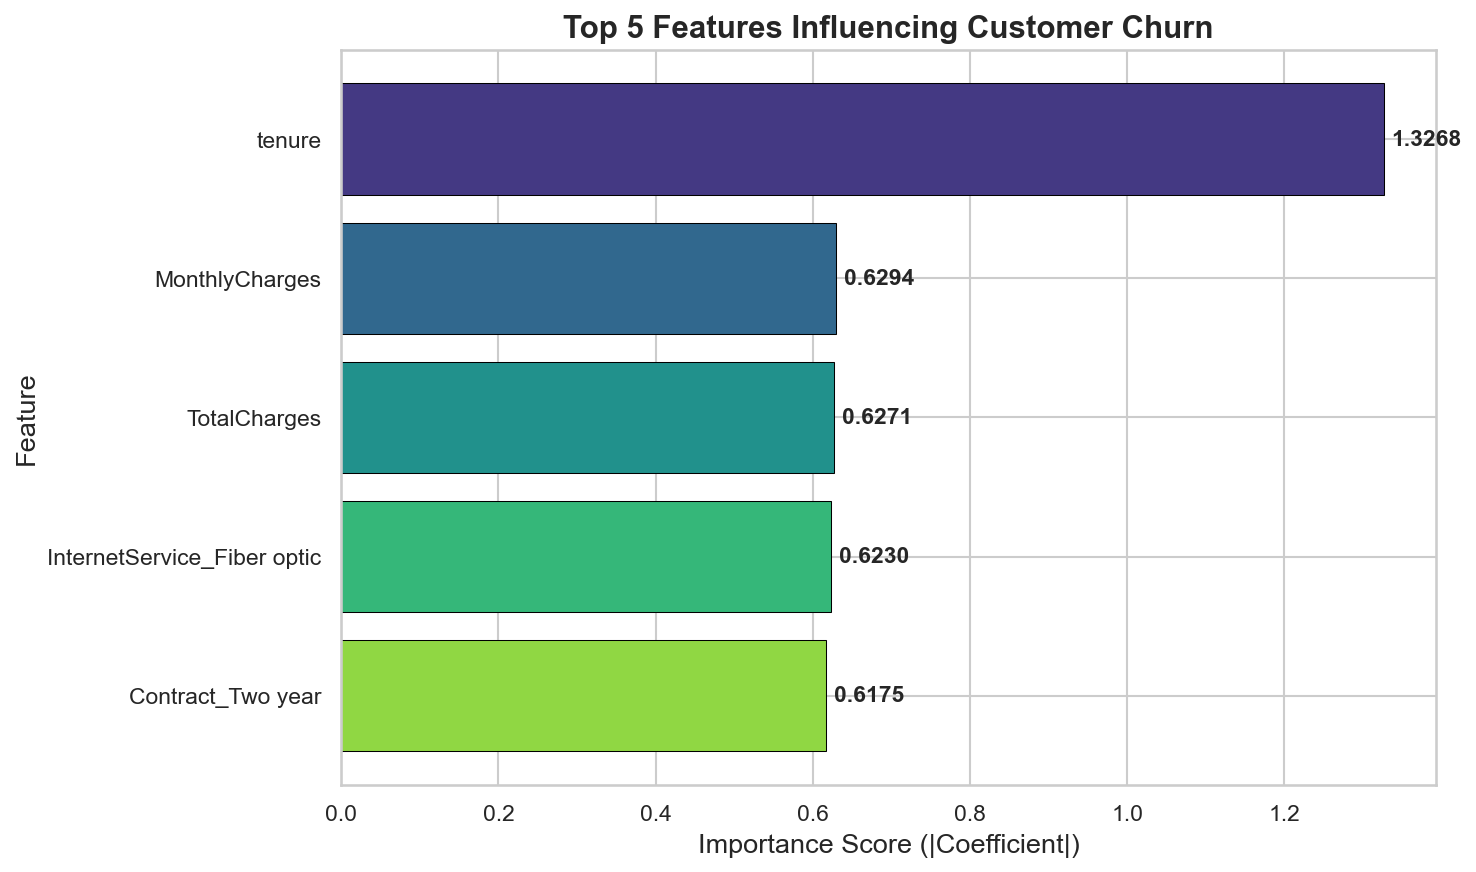
\includegraphics[width=0.48\textwidth]{../feature_importance.png}
  \caption{Global feature importance from the Gradient Boosting
           production model. Features are ranked by mean absolute
           SHAP value across the test set.}
  \label{fig:feature_importance}
\end{figure}

The top five churn drivers are:
\begin{enumerate}
  \item \textbf{Contract\_Two year} — Strongest \textit{retention} signal;
        two-year contracts reduce churn probability substantially.
  \item \textbf{Tenure} — Inverse relationship; new customers (low tenure)
        are disproportionately likely to churn in months 1–6.
  \item \textbf{InternetService\_Fiber optic} — Positive churn driver;
        Fiber customers show higher dissatisfaction, likely price-related.
  \item \textbf{MonthlyCharges} — Higher charges elevate churn risk,
        especially when tenure is low.
  \item \textbf{PaperlessBilling\_Yes} — Correlated with digital-native
        customers who face fewer switching barriers.
\end{enumerate}

Figure~\ref{fig:shap_bee} shows the SHAP beeswarm plot for the production
model on the test set, illustrating how each feature pushes predictions
towards churn (positive SHAP) or retention (negative SHAP) for every
individual customer.

\begin{figure}[H]
  \centering
  \includegraphics[width=0.48\textwidth]{figures/shap_beeswarm.png}
  \caption{SHAP beeswarm summary plot. Each point represents one customer
           in the test set. Red indicates high feature value; blue
           indicates low. Long-tenure, two-year-contract customers (blue
           dots, left) are strongly predicted as non-churners.}
  \label{fig:shap_bee}
\end{figure}

\subsection{Dashboard — Executive Summary View}

Figure~\ref{fig:dashboard} shows the Streamlit Executive Dashboard after
uploading a customer CSV, displaying live KPI cards and risk
segmentation charts.

\begin{figure}[H]
  \centering
  \includegraphics[width=0.48\textwidth]{figures/dashboard_screenshot.png}
  \caption{ChurnGuard AI Streamlit dashboard — Executive Summary tab.
           KPI cards show total customers, predicted churn rate, high-risk
           count, and average churn probability.}
  \label{fig:dashboard}
\end{figure}

% ============================================================
\section{Discussion}
% ============================================================

\subsection{Model Selection Rationale}

Gradient Boosting was chosen over Logistic Regression as the production
model despite LR's higher Recall (83.38\% vs 73.73\%), because its
extreme false-positive rate (37.4\% of non-churners flagged) would
overwhelm retention teams with non-actionable alerts. GB provides a
superior precision–recall operating point: with 275 true churners caught
and only 187 false alarms, each intervention is more likely to target
a genuine at-risk customer.

Logistic Regression remains available in the system as the
\textit{explainability} backbone — its linear coefficients are used to
generate the global feature importance chart in the dashboard.

\subsection{Class Imbalance Handling}

The 73.5\,:\,26.5 imbalance was addressed via:
\begin{itemize}
  \item \texttt{class\_weight=\char`"balanced\char`"} in LR — up-weights
        minority class samples in the loss function.
  \item Stratified splitting — ensures both splits preserve the 26.5\%
        churn prevalence.
  \item Threshold-aware evaluation — Recall and F1 are reported in
        addition to Accuracy to prevent the accuracy paradox.
\end{itemize}

\subsection{Limitations}

\begin{itemize}
  \item The model was trained on a single, US-centric telecom dataset;
        generalisation to other geographies or service types is not
        guaranteed.
  \item \texttt{TotalCharges} introduces temporal leakage risk (high
        correlation with \texttt{tenure} × \texttt{MonthlyCharges}).
  \item The LLM retention strategy quality depends on Groq API
        availability; the deterministic fallback is less nuanced.
\end{itemize}

% ============================================================
\section{Milestone 2: Agentic AI Retention System}
% ============================================================

\subsection{Architecture Overview}

Milestone 2 wraps the ML pipeline with a multi-node LangGraph
\cite{langgraph2024} StateGraph that accepts a selected customer record
and produces a structured retention strategy. The graph executes three
nodes sequentially:

\begin{center}
\footnotesize
\begin{tabular}{c}
\texttt{analyze\_risk} $\rightarrow$ \texttt{identify\_factors} \\
$\rightarrow$ \texttt{generate\_strategy} $\rightarrow$ \texttt{END}
\end{tabular}
\end{center}

Figure~\ref{fig:agent_arch} illustrates the full Milestone 2 pipeline.

\begin{figure}[H]
  \centering
  \includegraphics[width=0.48\textwidth]{figures/agent_pipeline.png}
  \caption{Milestone 2 agentic pipeline. SHAP attributions and RAG
           context feed into the LangGraph StateGraph, which calls the
           Groq LLM at each node to produce a structured
           \texttt{RetentionReport} validated by Pydantic v2.}
  \label{fig:agent_arch}
\end{figure}

\subsection{LLM Integration}

The Groq API \cite{groq2024} (\texttt{llama3-70b-8192}) provides
ultra-low-latency inference ($<$200\,ms per call). All three nodes
submit structured prompts and receive JSON responses validated against a
Pydantic \texttt{RetentionReport} schema:

\begin{lstlisting}[language=Python, caption={Pydantic schema for structured LLM output}]
class ActionItem(BaseModel):
    action:    str
    rationale: str
    priority:  Literal["High","Medium","Low"]

class RetentionReport(BaseModel):
    risk_level:           str
    risk_summary:         str
    churn_probability:    float
    contributing_factors: List[str]
    recommended_actions:  List[ActionItem]
    sources:              List[str]
    disclaimers:          List[str]
\end{lstlisting}

If JSON parsing fails, the node retries once with an explicit correction
prompt. If the Groq API is unavailable, a deterministic rule-based
fallback fires automatically.

\vspace{0.5em}
\subsection{RAG Pipeline}
\vspace{0.3em}

A lightweight Retrieval-Augmented Generation pipeline \cite{lewis2020rag}
provides domain-specific context to the \texttt{generate\_strategy} node:

\begin{itemize}
  \item \textbf{Corpus}: A curated knowledge base of telecom retention
        playbooks stored in \texttt{data/knowledge\_base/}.
  \item \textbf{Embeddings}: \texttt{all-MiniLM-L6-v2}
        \cite{reimers2019sentencebert} via \texttt{sentence-transformers}.
  \item \textbf{Vector store}: ChromaDB \cite{chromadb2023}, persisted
        locally under \texttt{data/chromadb/}.
  \item \textbf{Retrieval}: Top-3 most semantically similar passages are
        appended to the strategy-generation prompt as context.
\end{itemize}

\subsection{SHAP Integration}

Per-customer SHAP values (linear surrogate, kernel background of 100
training samples) are computed before the agent call and injected into
the \texttt{identify\_factors} prompt, ensuring the LLM's stated
contributing factors are grounded in the model's actual decision logic
rather than hallucinated generalisations.

\subsection{Extension Features}

\subsubsection*{PDF Export}
Using \texttt{fpdf2} \cite{fpdf2}, the system generates a professionally
formatted retention report (header, customer profile table, risk
assessment, ranked action items, disclaimers, timestamp) as a
downloadable PDF via \texttt{st.download\_button()}.

\subsubsection*{Batch Analytics Dashboard}
A dedicated tab provides portfolio-level analytics:
\begin{itemize}
  \item \textbf{Risk donut chart} — High / Medium / Low customer counts.
  \item \textbf{Segment breakdown} — Churn rate by Contract type,
        Internet Service, and Payment Method.
  \item \textbf{Tenure × Charges heatmap} — Average churn probability
        across binned tenure and monthly-charge dimensions.
  \item \textbf{Top-20 at-risk table} — Ranked by churn probability with
        key attributes.
\end{itemize}

\subsection{AI Advisor Output Example}

Figure~\ref{fig:advisor} shows the AI Retention Advisor tab after
selecting a high-risk customer, displaying the structured LLM output.

\begin{figure}[H]
  \centering
  \includegraphics[width=0.48\textwidth]{figures/ai_advisor_screenshot.png}
  \caption{AI Retention Advisor tab showing the structured output for a
           selected high-risk customer: risk level badge, risk summary,
           contributing factors, and prioritised recommended actions.}
  \label{fig:advisor}
\end{figure}

% ============================================================
\section{Conclusion}
% ============================================================

This paper presented ChurnGuard AI, an end-to-end system for telecom
customer churn prediction and AI-driven retention. The key contributions
are:

\begin{enumerate}
  \item A rigorous three-model ML comparison on the IBM Telco dataset,
        establishing Gradient Boosting as the optimal production model
        (F1~=~65.87\%, AUC~=~0.860).
  \item SHAP-based local and global explainability, enabling
        non-technical stakeholders to understand \textit{why} a customer
        is flagged as at risk.
  \item A LangGraph agentic workflow that chains LLM calls with RAG
        retrieval to produce structured, Pydantic-validated retention
        strategies grounded in customer-specific SHAP attributions.
  \item Two extension features — PDF export and a batch analytics
        dashboard — that increase the system's practical utility for
        operations and management teams.
\end{enumerate}

\textbf{Future work} includes: (i) experimentation with
XGBoost~\cite{chen2016xgboost} and class-balancing via SMOTE
\cite{chawla2002smote}; (ii) online learning to retrain the model
incrementally as new data arrives; (iii) CRM integration so
agent-recommended actions automatically create support tickets; and
(iv) A/B testing of retention interventions to close the feedback loop
between prediction and business outcome.

% ============================================================
%  References
% ============================================================
\bibliographystyle{IEEEtranN}

\begin{thebibliography}{99}

\bibitem{reichheld1990zero}
F.~F. Reichheld and W.~E. Sasser,
``Zero defections: Quality comes to services,''
\textit{Harvard Business Review}, vol.~68, no.~5, pp.~105--111, 1990.

\bibitem{statista2024telecom}
Statista Research Department,
``Global telecommunications market revenue 2018--2026,''
Statista, 2024. [Online].
Available: \url{https://www.statista.com/statistics/263438/revenue-of-the-global-telecommunication-industry/}

\bibitem{vafeiadis2015comparison}
T.~Vafeiadis, K.~I. Diamantaras, G.~Sarigiannidis, and S.~K. Chatzisavvas,
``A comparison of machine learning techniques for customer churn prediction,''
\textit{Simulation Modelling Practice and Theory}, vol.~55, pp.~1--9, 2015.

\bibitem{umayaparvathi2016attribute}
V.~Umayaparvathi and K.~Iyakutti,
``Attribute selection and customer churn prediction in telecom industry,''
in \textit{Proc. Int. Conf. Data Mining and Advanced Computing}, 2016,
pp.~1--5.

\bibitem{kirui2013predicting}
C.~Kirui, L.~Hong, W.~Cheruiyot, and H.~Kirui,
``Predicting customer churn in mobile telephony industry using probabilistic
classifiers in data mining,''
\textit{International Journal of Computer Science and Information Technology},
vol.~5, no.~2, pp.~165--172, 2013.

\bibitem{lundberg2017shap}
S.~M. Lundberg and S.~Lee,
``A unified approach to interpreting model predictions,''
in \textit{Advances in Neural Information Processing Systems}, vol.~30,
pp.~4765--4774, 2017.

\bibitem{lewis2020rag}
P.~Lewis \textit{et al.},
``Retrieval-augmented generation for knowledge-intensive NLP tasks,''
in \textit{Advances in Neural Information Processing Systems}, vol.~33,
pp.~9459--9474, 2020.

\bibitem{kaggle_telco}
IBM,
``Telco customer churn dataset,''
Kaggle, 2018. [Online].
Available: \url{https://www.kaggle.com/datasets/blastchar/telco-customer-churn}

\bibitem{langgraph2024}
LangChain Inc.,
``LangGraph: Build stateful, multi-actor applications with LLMs,''
2024. [Online].
Available: \url{https://langchain-ai.github.io/langgraph/}

\bibitem{groq2024}
Groq Inc.,
``Groq API documentation,''
2024. [Online].
Available: \url{https://console.groq.com/docs}

\bibitem{reimers2019sentencebert}
N.~Reimers and I.~Gurevych,
``Sentence-BERT: Sentence embeddings using Siamese BERT-networks,''
in \textit{Proc. Conf. on Empirical Methods in Natural Language Processing
(EMNLP)}, 2019, pp.~3982--3992.

\bibitem{chromadb2023}
Chroma,
``ChromaDB: The AI-native open-source embedding database,''
2023. [Online].
Available: \url{https://www.trychroma.com}

\bibitem{fpdf2}
O.~Gustafsson \textit{et al.},
``fpdf2: PDF generation library for Python,''
2023. [Online].
Available: \url{https://pyfpdf.github.io/fpdf2/}

\bibitem{chen2016xgboost}
T.~Chen and C.~Guestrin,
``XGBoost: A scalable tree boosting system,''
in \textit{Proc. 22nd ACM SIGKDD Int. Conf. Knowledge Discovery and Data
Mining}, 2016, pp.~785--794.

\bibitem{chawla2002smote}
N.~V. Chawla, K.~W. Bowyer, L.~O. Hall, and W.~P. Kegelmeyer,
``SMOTE: Synthetic minority over-sampling technique,''
\textit{Journal of Artificial Intelligence Research}, vol.~16,
pp.~321--357, 2002.

\bibitem{pedregosa2011sklearn}
F.~Pedregosa \textit{et al.},
``Scikit-learn: Machine learning in Python,''
\textit{Journal of Machine Learning Research}, vol.~12, pp.~2825--2830,
2011.

\end{thebibliography}

% ============================================================
%  Appendix
% ============================================================
\appendix

\section{GitHub Repository}

The complete source code, trained models, notebooks, and documentation
are publicly available at:

\begin{center}
\textbf{\url{https://github.com/ANANYA542/AI-ML-Churn_detection}}
\end{center}

\subsection{Repository Structure}

\begin{verbatim}
AI-ML-Churn_detection/
├── app.py                  # Streamlit entry point
├── requirements.txt        # Python dependencies
├── feature_importance.png  # Global feature importance
├── .streamlit/config.toml  # UI theme
├── src/
│   ├── agent.py            # LangGraph agent workflow
│   ├── llm_client.py       # Groq API wrapper
│   ├── pdf_export.py       # fpdf2 PDF generator
│   ├── processor.py        # Data preprocessing
│   ├── explainability.py   # SHAP integration
│   ├── rag.py              # ChromaDB RAG pipeline
│   ├── ui_components.py    # Streamlit rendering functions
│   └── model_loader.py     # Model/scaler/metrics loader
├── models/
│   ├── model.pkl           # Gradient Boosting (production)
│   ├── best_model.pkl      # Best model from comparison
│   ├── scaler.pkl          # StandardScaler
│   ├── feature_names.pkl   # Ordered feature list
│   ├── metrics.json        # Production model metrics
│   └── comparison.json     # All-model comparison metrics
├── data/
│   ├── telco.csv           # Raw IBM Telco dataset
│   ├── chromadb/           # Persisted ChromaDB vector store
│   └── knowledge_base/     # RAG corpus (text files)
├── notebooks/
│   ├── preprocessing.ipynb
│   ├── model_training.ipynb
│   ├── model_comparison.ipynb
│   └── feature_importance.ipynb
└── report/
    └── main.tex            # This document
\end{verbatim}

\subsection{Reproducing Results}

\begin{lstlisting}[language=bash, caption={Setup and run instructions}]
git clone https://github.com/ANANYA542/AI-ML-Churn_detection.git
cd AI-ML-Churn_detection
python -m venv .venv && source .venv/bin/activate
pip install -r requirements.txt
# Add GROQ_API_KEY to .env
streamlit run app.py
\end{lstlisting}

\section{Note on Figures}

All screenshots and generated plots used in this report should be
placed in a \texttt{figures/} subdirectory alongside this \texttt{.tex}
file before compiling. The required files are:

\begin{itemize}
  \item \texttt{figures/churn\_distribution.png} — Bar/pie chart of
        Churn Yes/No counts (generate from \texttt{preprocessing.ipynb})
  \item \texttt{figures/confusion\_matrices.png} — Side-by-side
        heatmaps for LR, RF, GB (from \texttt{model\_comparison.ipynb})
  \item \texttt{figures/roc\_curves.png} — Overlaid ROC curves
        (from \texttt{model\_comparison.ipynb})
  \item \texttt{figures/shap\_beeswarm.png} — SHAP beeswarm summary
        (from \texttt{feature\_importance.ipynb})
  \item \texttt{figures/agent\_pipeline.png} — Architecture diagram
        (draw in draw.io or similar)
  \item \texttt{figures/dashboard\_screenshot.png} — Streamlit UI
        screenshot
  \item \texttt{figures/ai\_advisor\_screenshot.png} — AI Advisor tab
        screenshot
\end{itemize}

\end{document}
